\documentclass[fleqn]{goose-article}

\title{Energy barrier}
\author{Tom de Geus}
\hypersetup{pdfauthor={T.W.J. de Geus}}

\begin{document}

\maketitle

\section*{Protocol}

The protocol is as follows.
\begin{enumerate}
    \item An element is selected for triggering
    (in the example below chosen in the center of the system).
    Its location is denoted by $\vec{r}'$.

    \item A perturbation around a stress and strain free configuration is considered.
    To this end, the selected element (only) is subjected to an eigen stress
    $\bm{\sigma}'$.
    The corresponding equilibrium configuration then constitutes to
    the perturbation that will be used.
    It is characterised by the stress field $\vec{u}^* (\vec{r})$, and corresponding
    stress $\bm{\sigma}^* (\vec{r})$
    and strain $\bm{\varepsilon}^* (\vec{r})$ fields.

    \item Two types of perturbations are considered:
    \begin{itemize}
        \item Simple shear:
        $\bm{\sigma}' = \bm{\sigma}'_s = \vec{e}_x \vec{e}_y + \vec{e}_x \vec{e}_y$.
        Gives: $\vec{u}^*_s (\vec{r})$, $\bm{\sigma}^*_s (\vec{r})$, and
        $\bm{\varepsilon}^*_s (\vec{r})$.

        \item Pure shear:
        $\bm{\sigma}' = \bm{\sigma}'_p = \vec{e}_x \vec{e}_x - \vec{e}_y \vec{e}_y$.
        Gives: $\vec{u}^*_p (\vec{r})$, $\bm{\sigma}^*_p (\vec{r})$, and
        $\bm{\varepsilon}^*_p (\vec{r})$.
    \end{itemize}

    For the triggered element the strain (and) stress are (by definition)
    of the following structure:
    $\bm{\varepsilon}^*_s (\vec{r}') = \chi_s (\vec{e}_x \vec{e}_y + \vec{e}_x \vec{e}_y)$
    for the simple shear perturbation, and
    $\bm{\varepsilon}^*_p (\vec{r}') = \chi_p (\vec{e}_x \vec{e}_x - \vec{e}_y \vec{e}_y)$
    for the pure shear perturbation.

    \item A perturbation $\delta \vec{u}(\vec{r}) = s \vec{u}^*_s (\vec{r}) + p \vec{u}^*_p (\vec{r})$
    is then applied such that it results in the minimal increase of potential energy in the
    landscape.

\end{enumerate}

\begin{figure}[htp]
    \centering
    \captionsetup[subfigure]{justification=centering}
    \begin{minipage}[t]{.49\textwidth}
        \centering
        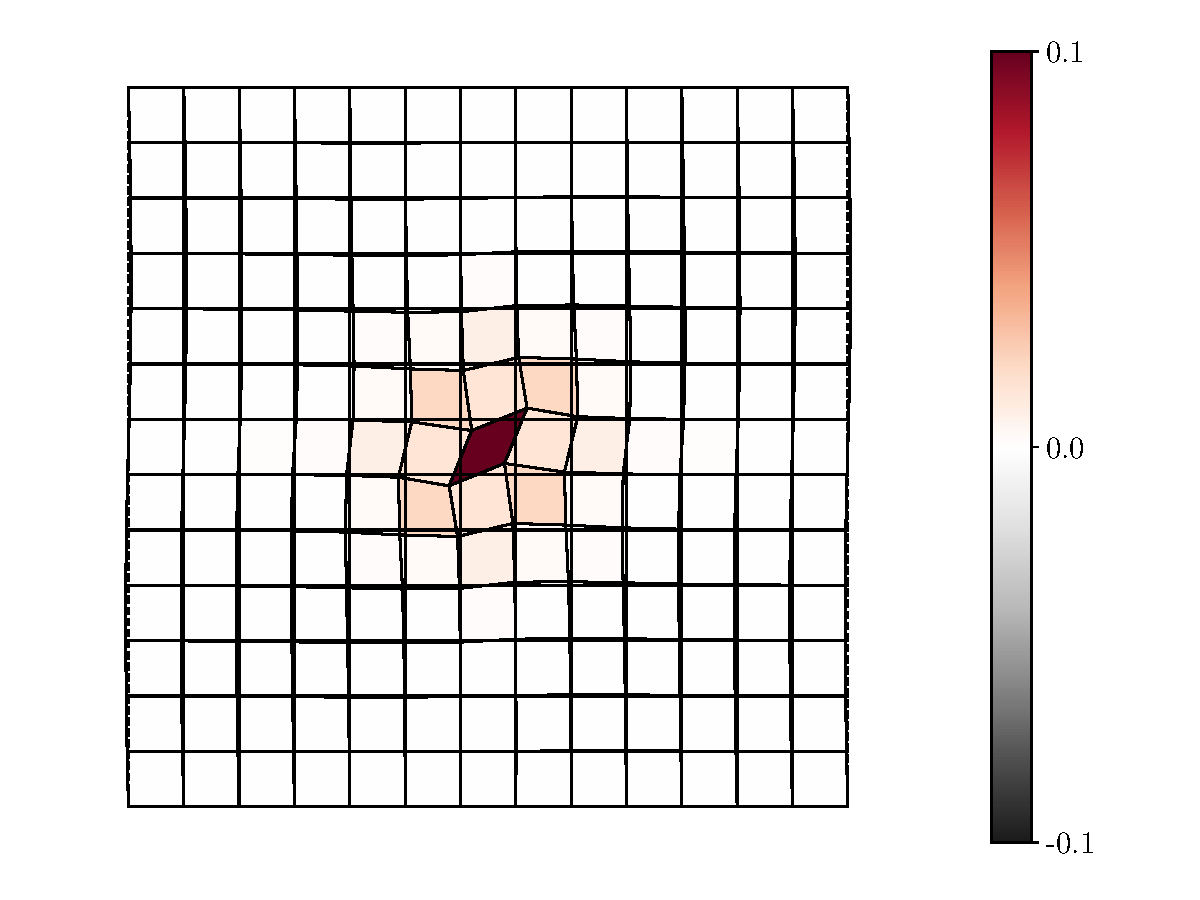
\includegraphics[width=\textwidth]{perturbation_simple-shear_energy.pdf}
        \subcaption{Simple shear}
        \label{fig:perturbation:simple-shear}
    \end{minipage}
    \hfill
    \begin{minipage}[t]{.49\textwidth}
        \centering
        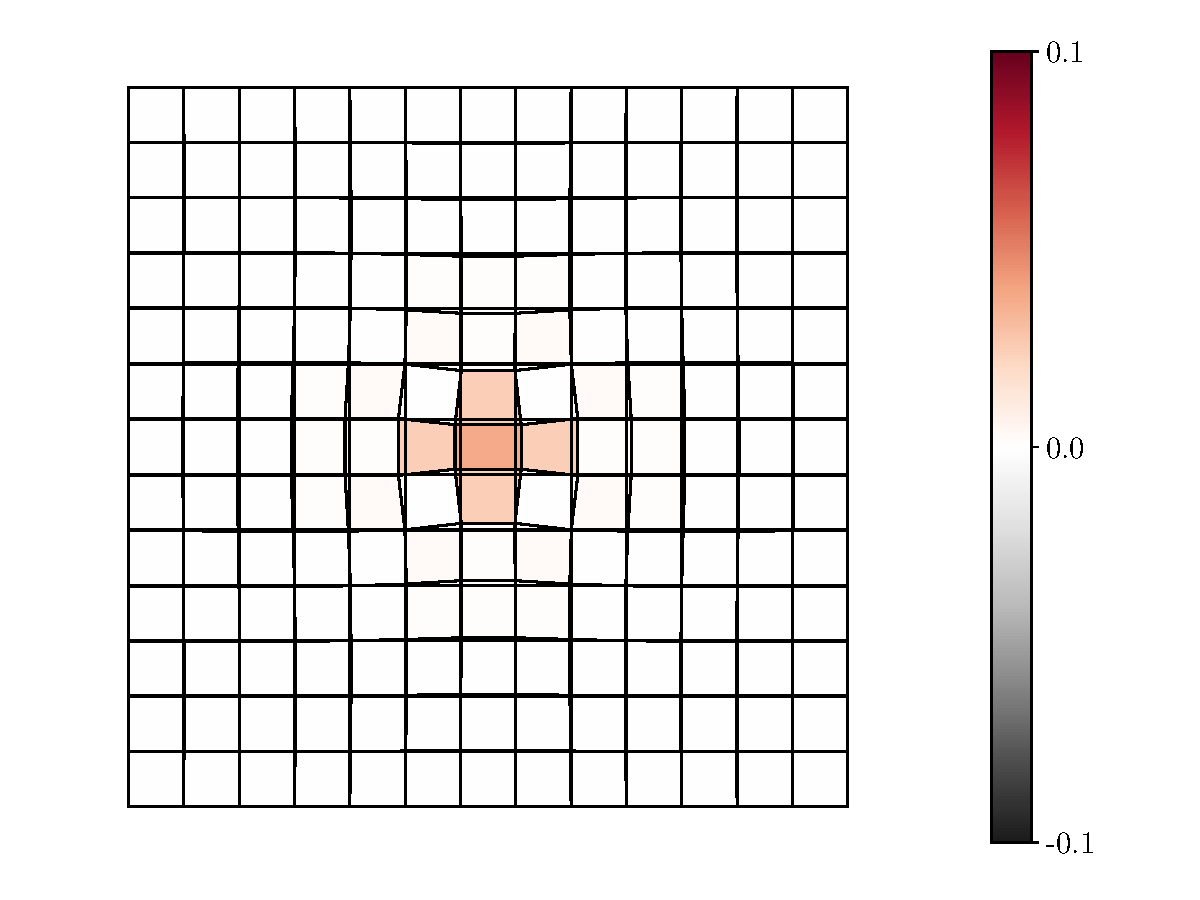
\includegraphics[width=\textwidth]{perturbation_pure-shear_energy.pdf}
        \subcaption{Pure shear}
        \label{fig:perturbation:pure-shear}
    \end{minipage}
    \caption{
        Perturbation modes.
        The shown colour is the energy change resulting from the perturbation.
    }
    \label{fig:perturbation}
\end{figure}

\begin{figure}[htp]
    \centering
    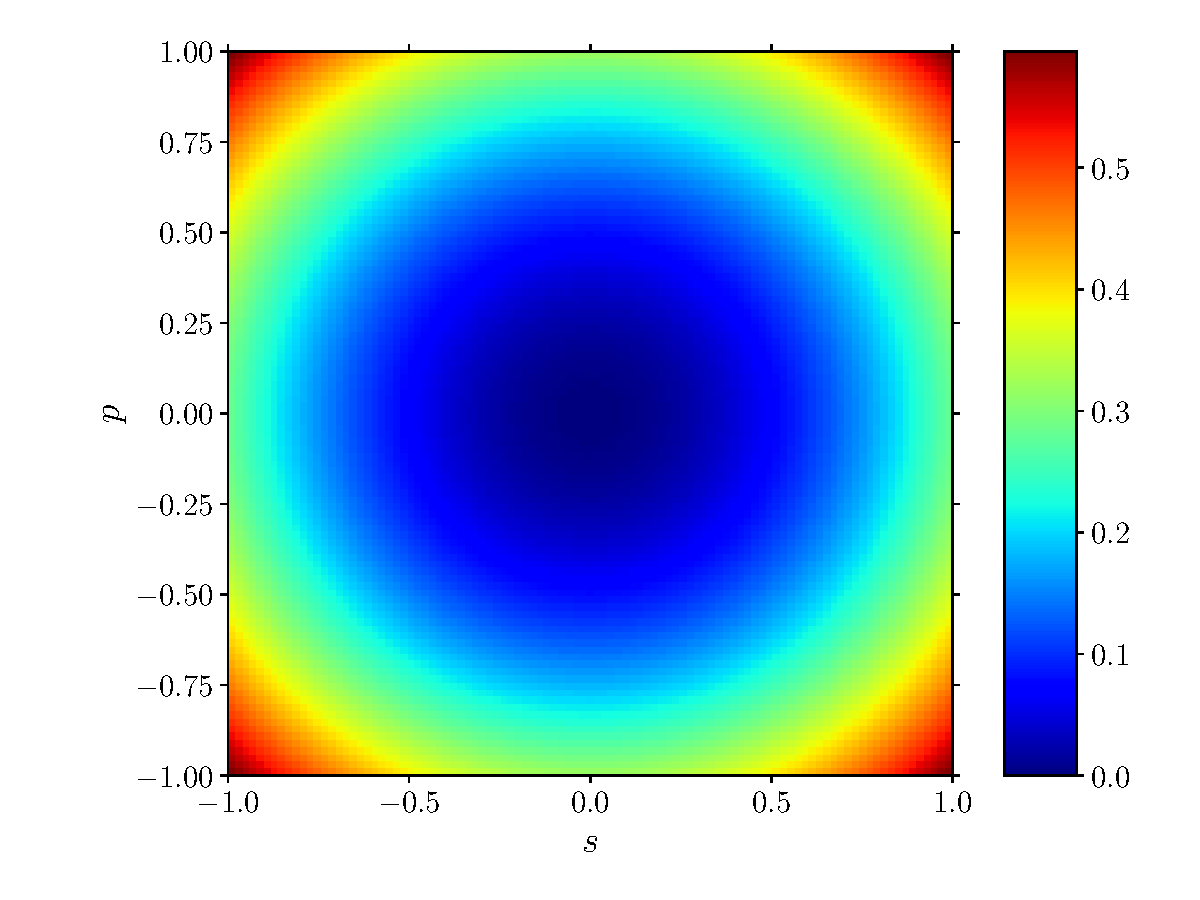
\includegraphics[width=.5\textwidth]{phase-diagram_energy.pdf}
    \caption{
        Energetic cost of a perturbation:
        $\delta \vec{u}(\vec{r}) = s \vec{u}^*_s (\vec{r}) + p \vec{u}^*_p (\vec{r})$.
    }
    \label{fig:energy}
\end{figure}

\begin{figure}[htp]
    \centering
    \captionsetup[subfigure]{justification=centering}
    \begin{minipage}[t]{.49\textwidth}
        \centering
        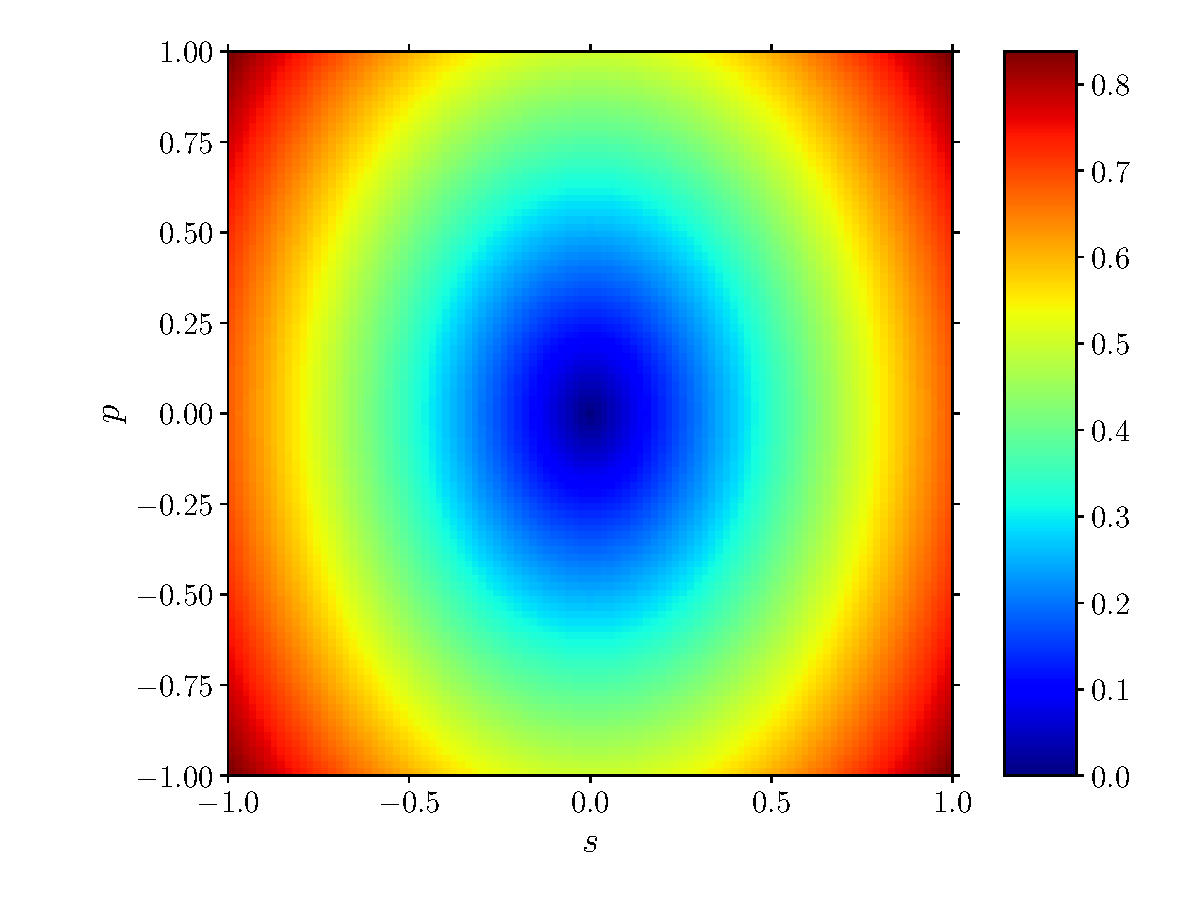
\includegraphics[width=\textwidth]{phase-diagram_sig.pdf}
        \subcaption{
            Equivalent stress.
        }
        \label{fig:phase-diagram:sig}
    \end{minipage}
    \hfill
    \begin{minipage}[t]{.49\textwidth}
        \centering
        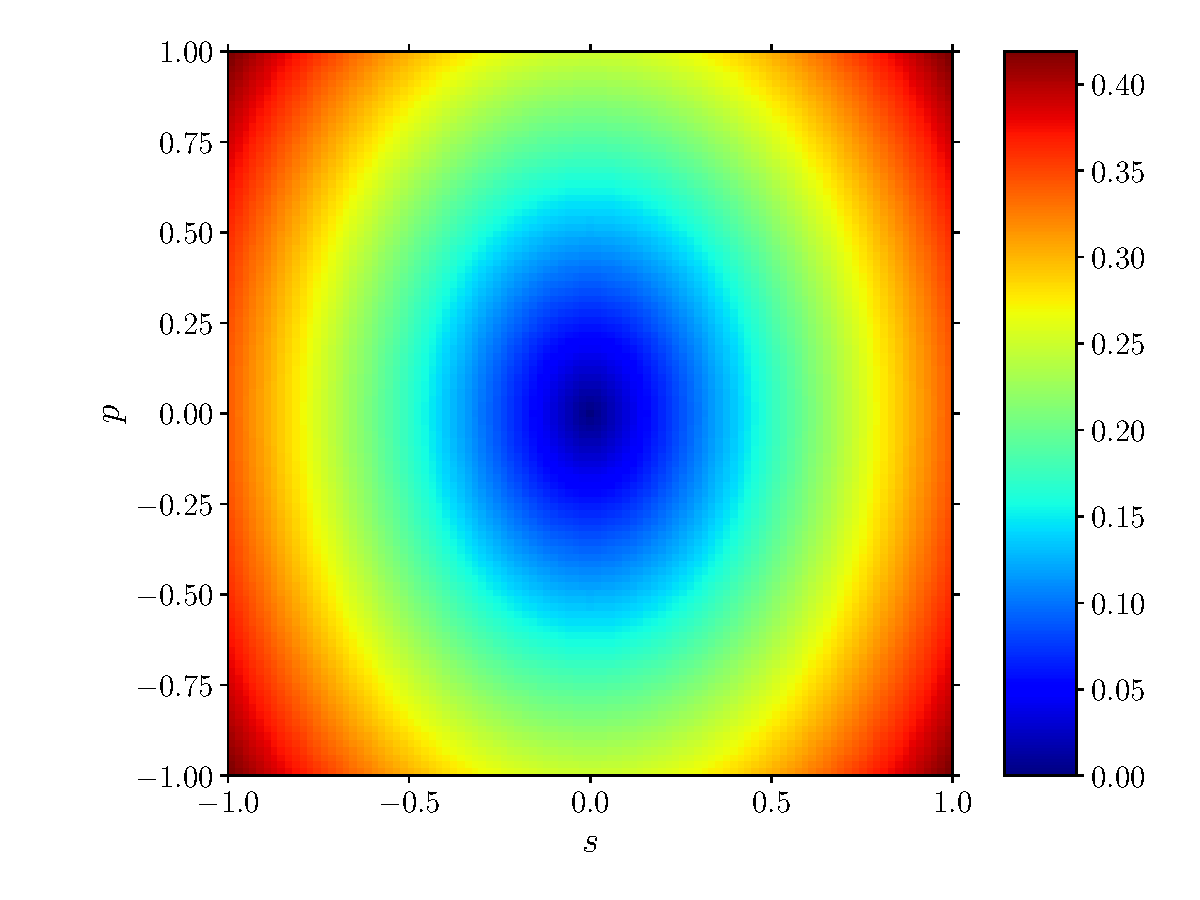
\includegraphics[width=\textwidth]{phase-diagram_eps.pdf}
        \subcaption{
            Equivalent strain.
        }
        \label{fig:phase-diagram:eps}
    \end{minipage}
    \caption{
        Resulting
        \subref{fig:phase-diagram:sig} equivalent stress and
        \subref{fig:phase-diagram:eps} equivalent strain
        for a perturbation:
        $\delta \vec{u}(\vec{r}) = s \vec{u}^*_s (\vec{r}) + p \vec{u}^*_p (\vec{r})$.
    }
    \label{fig:phase-diagram}
\end{figure}

\clearpage

\section*{Example}

An example for two configurations in \cref{fig:example:config} is shown in
\cref{fig:example:phase-diagram}.

\begin{figure}[htp]
    \centering
    \captionsetup[subfigure]{justification=centering}
    \begin{minipage}[t]{.40\textwidth}
        \centering
        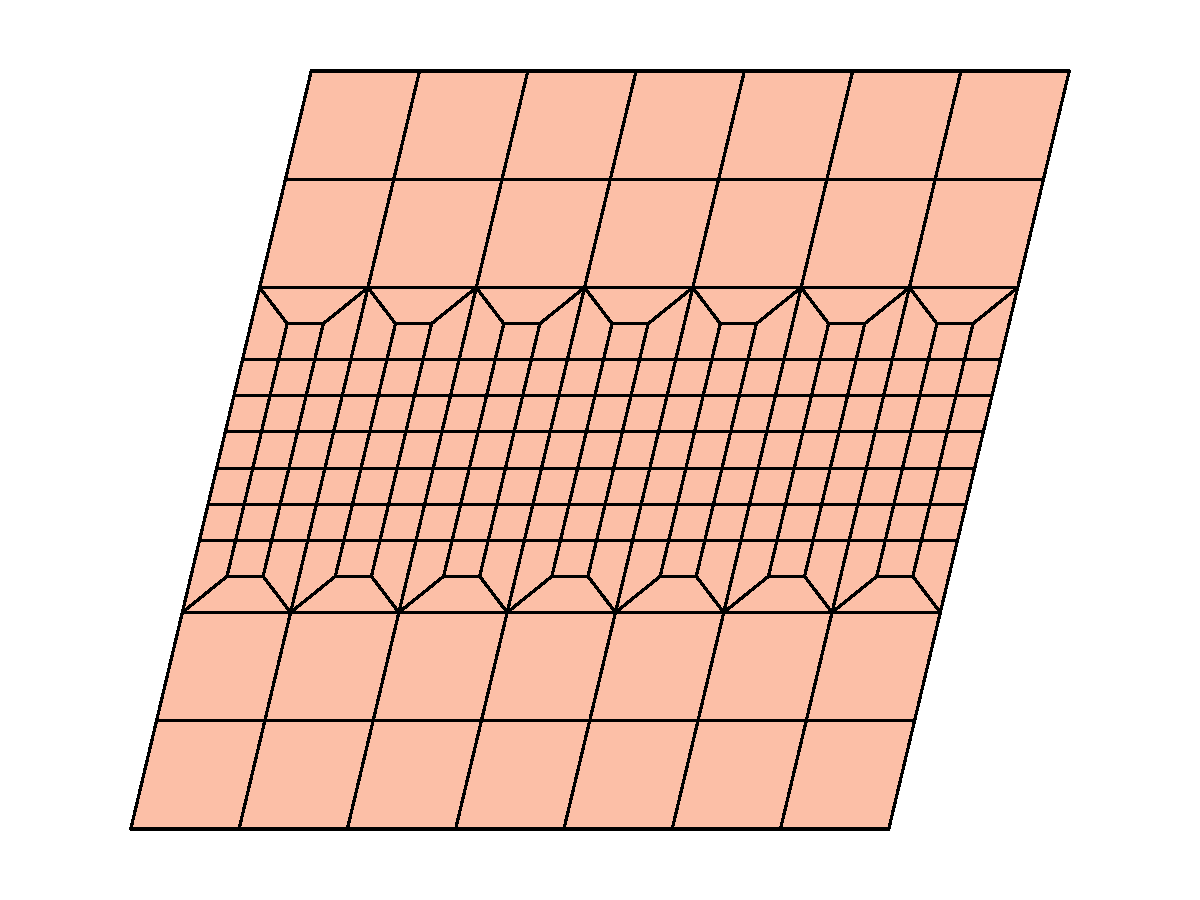
\includegraphics[width=\textwidth]{prestress_0_config.pdf}
        \subcaption{Initial configuration.}
    \end{minipage}
    \hspace{0.01\textwidth}
    \begin{minipage}[t]{.40\textwidth}
        \centering
        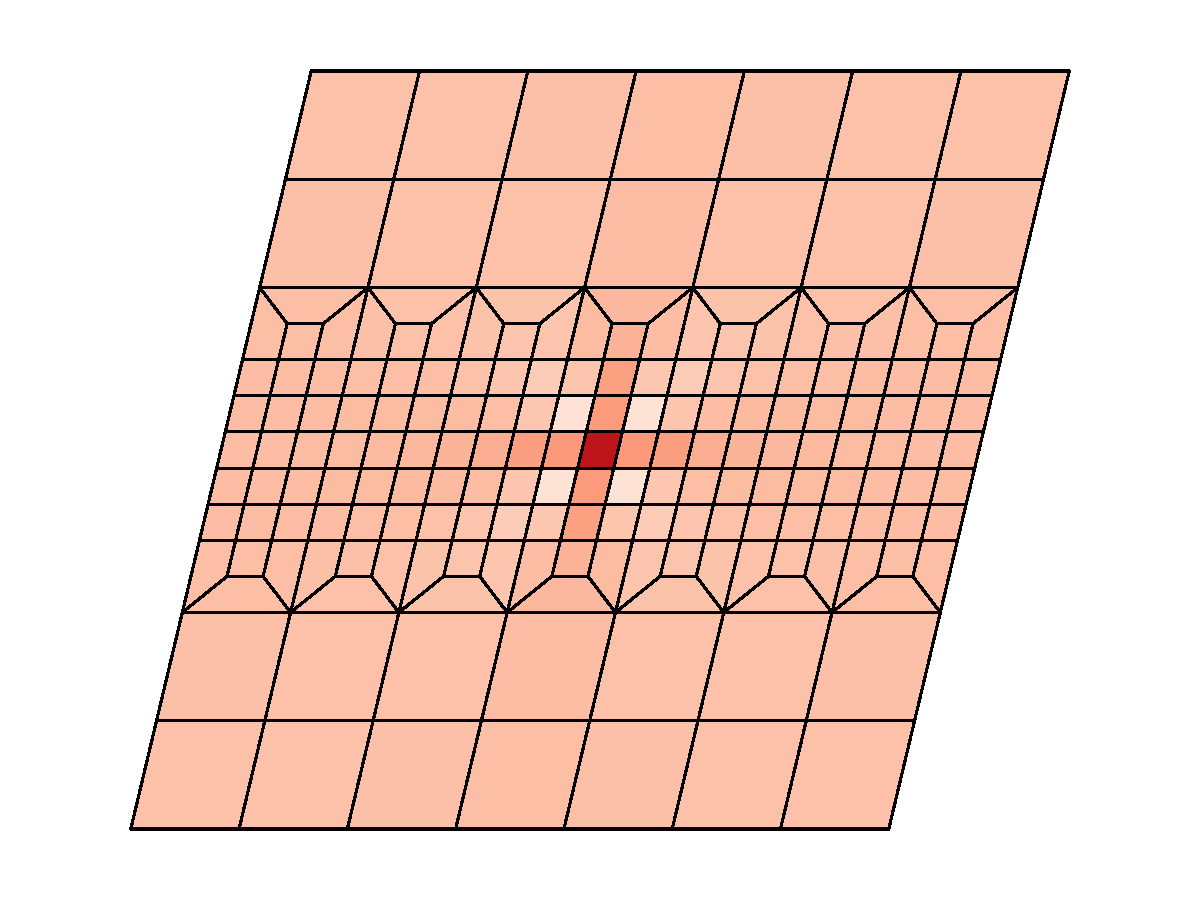
\includegraphics[width=\textwidth]{prestress_0_config-perturbed.pdf}
        \subcaption{After perturbation.}
    \end{minipage}
    \\
    \begin{minipage}[t]{.40\textwidth}
        \centering
        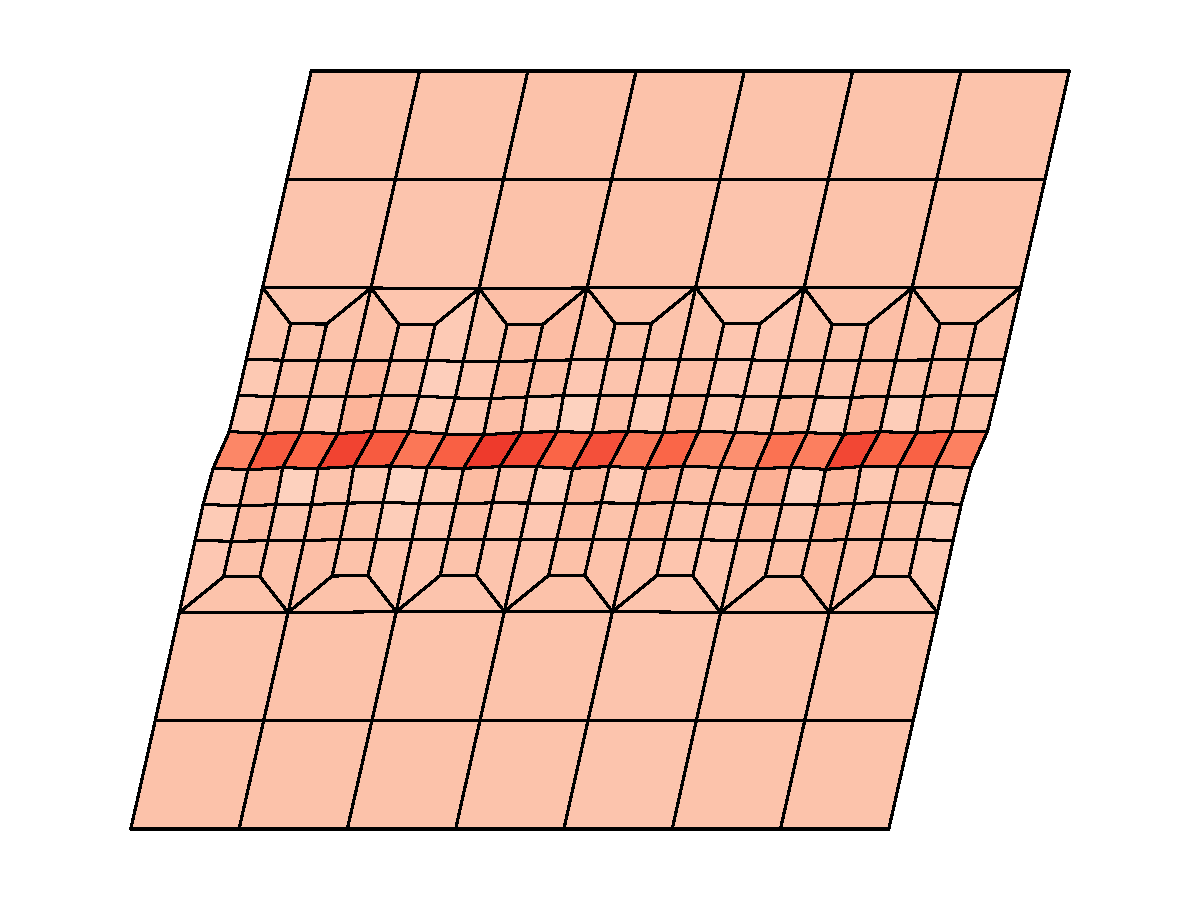
\includegraphics[width=\textwidth]{prestress_1_config.pdf}
        \subcaption{Initial configuration.}
    \end{minipage}
    \hspace{0.01\textwidth}
    \begin{minipage}[t]{.40\textwidth}
        \centering
        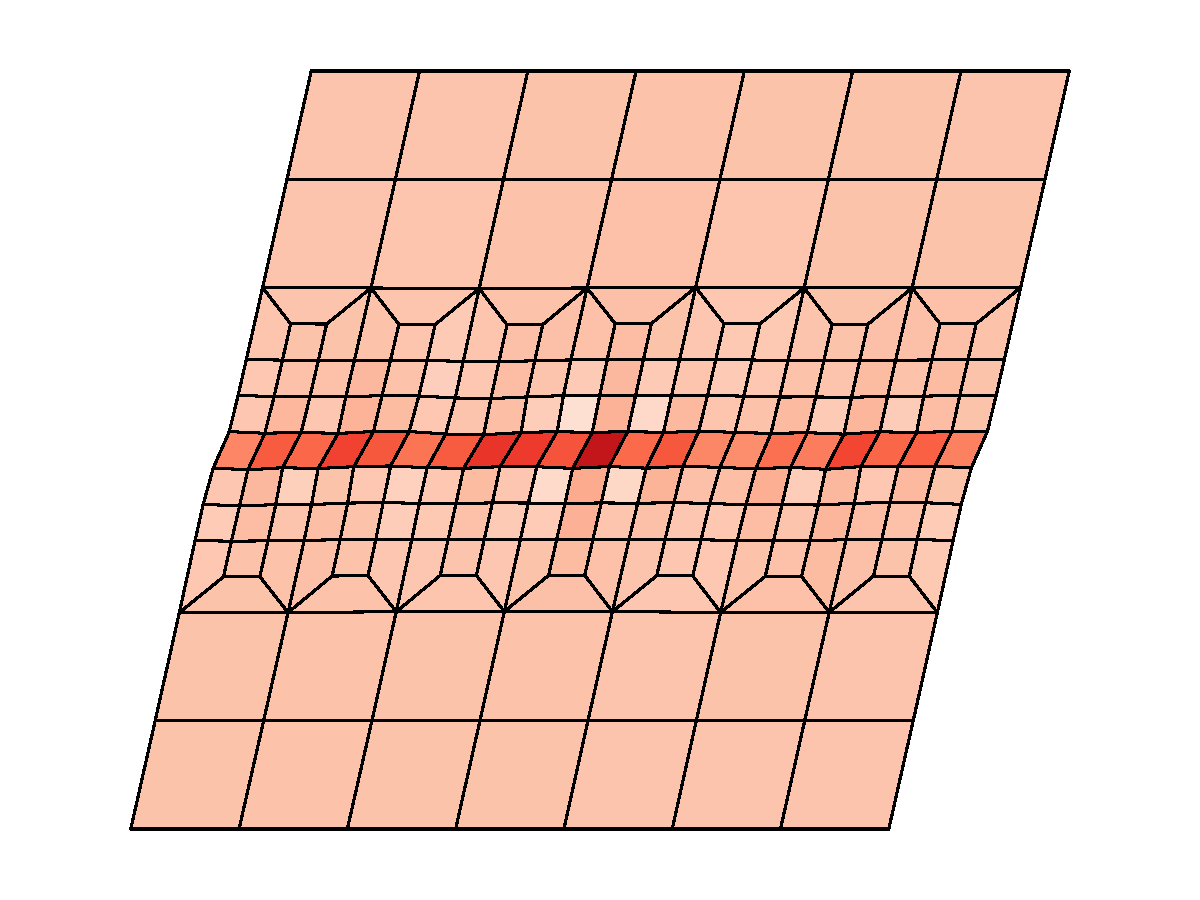
\includegraphics[width=\textwidth]{prestress_1_config-perturbed.pdf}
        \subcaption{After perturbation.}
    \end{minipage}
    \caption{
        Starting and perturbed configuration, for (a-b) a homogeneous sheared system, and
        (c-d) a homogeneous sheared system subjected to a random pre-stress.
    }
    \label{fig:example:config}
\end{figure}

\begin{figure}[htp]
    \centering
    \captionsetup[subfigure]{justification=centering}
    \begin{minipage}[t]{.31\textwidth}
        \centering
        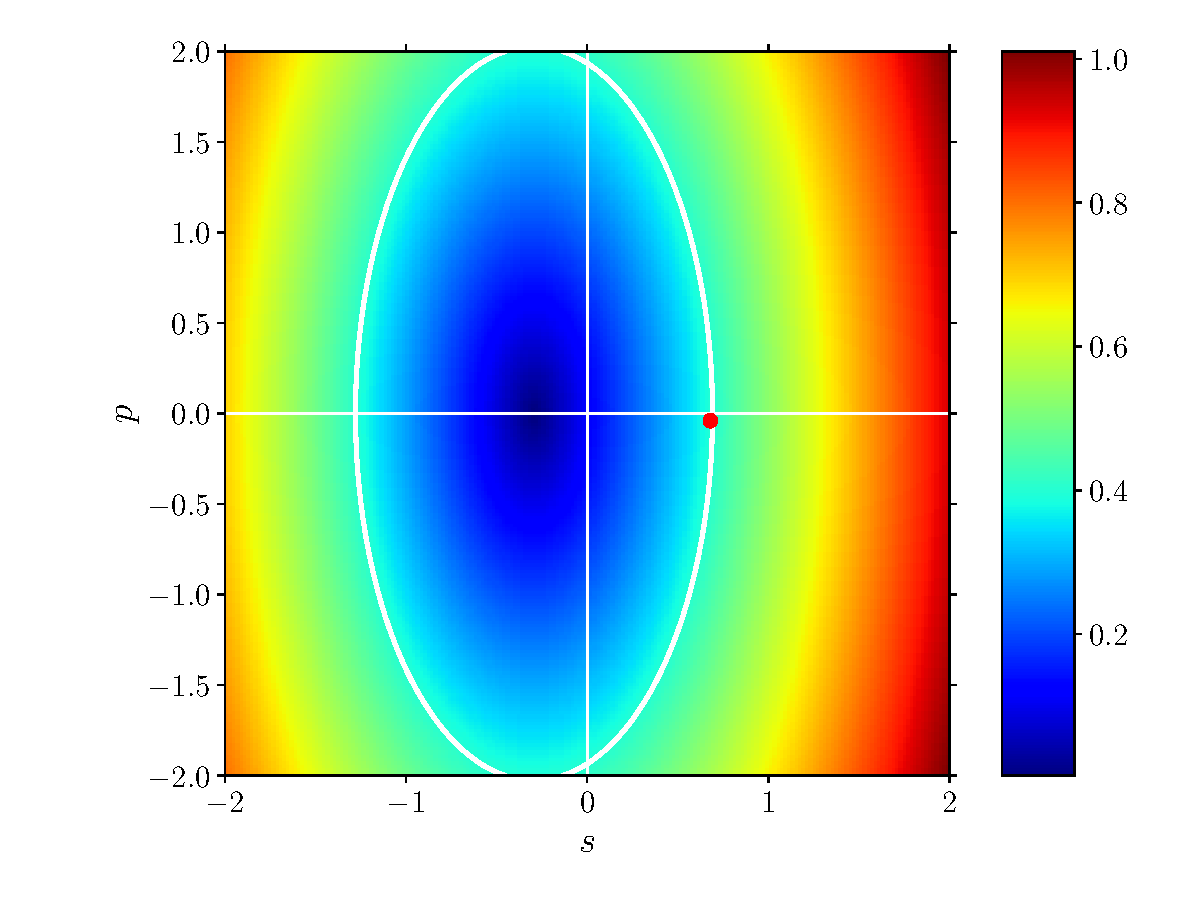
\includegraphics[width=\textwidth]{prestress_0_phase-diagram_eps.pdf}
        \subcaption{$\varepsilon$}
        \label{fig:}
    \end{minipage}
    \hfill
    \begin{minipage}[t]{.31\textwidth}
        \centering
        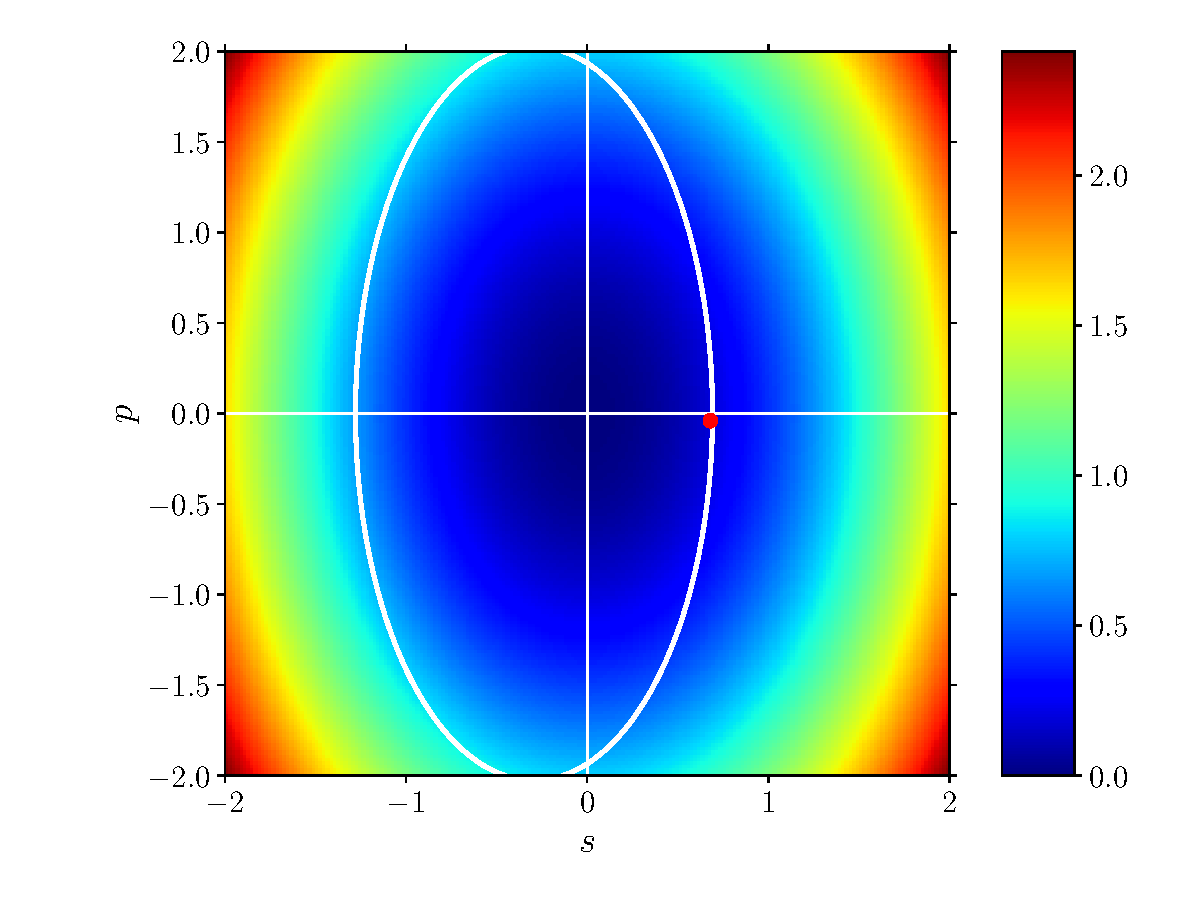
\includegraphics[width=\textwidth]{prestress_0_phase-diagram_energy.pdf}
        \subcaption{$\Delta E$}
        \label{fig:}
    \end{minipage}
    \hfill
    \begin{minipage}[t]{.31\textwidth}
        \centering
        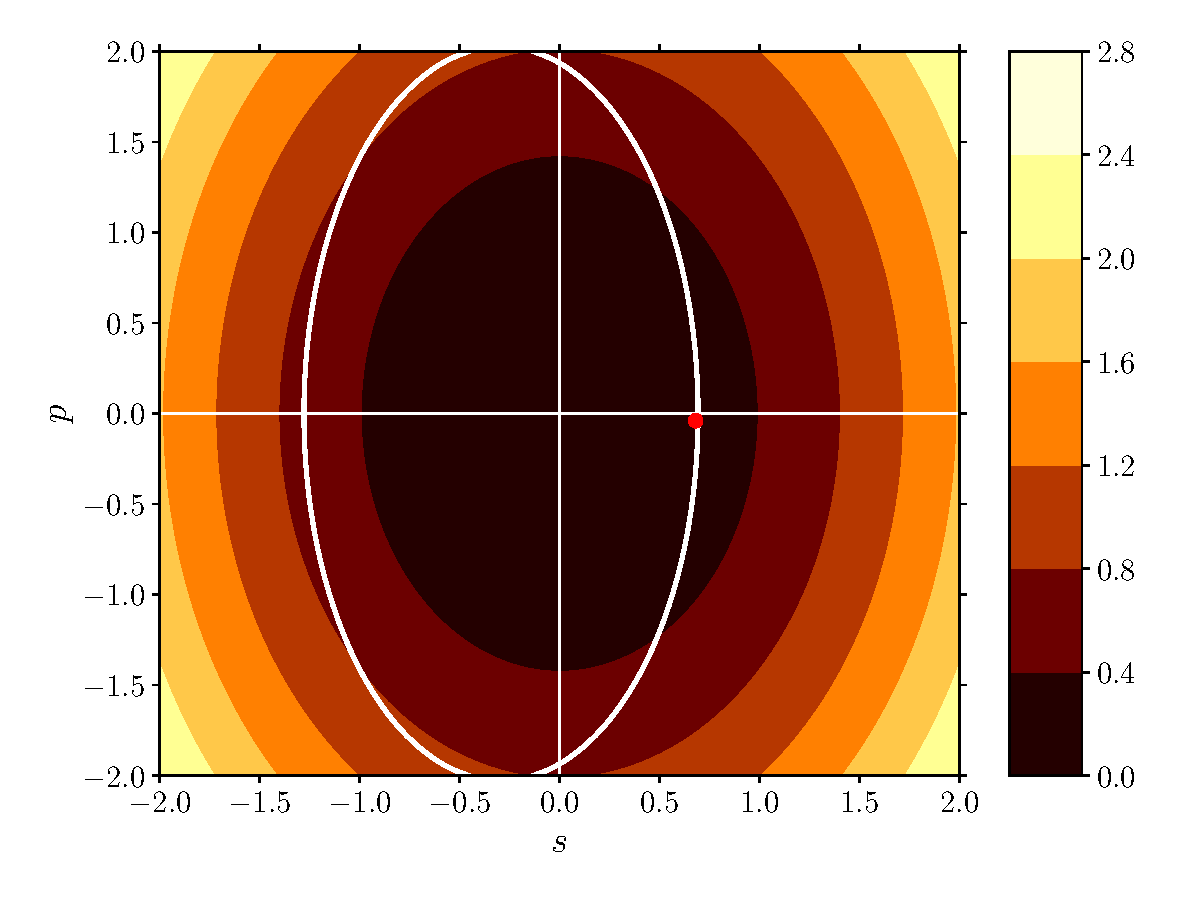
\includegraphics[width=\textwidth]{prestress_0_phase-diagram_energy-contour.pdf}
        \subcaption{$\Delta E$}
        \label{fig:}
    \end{minipage}
    \\
    \begin{minipage}[t]{.31\textwidth}
        \centering
        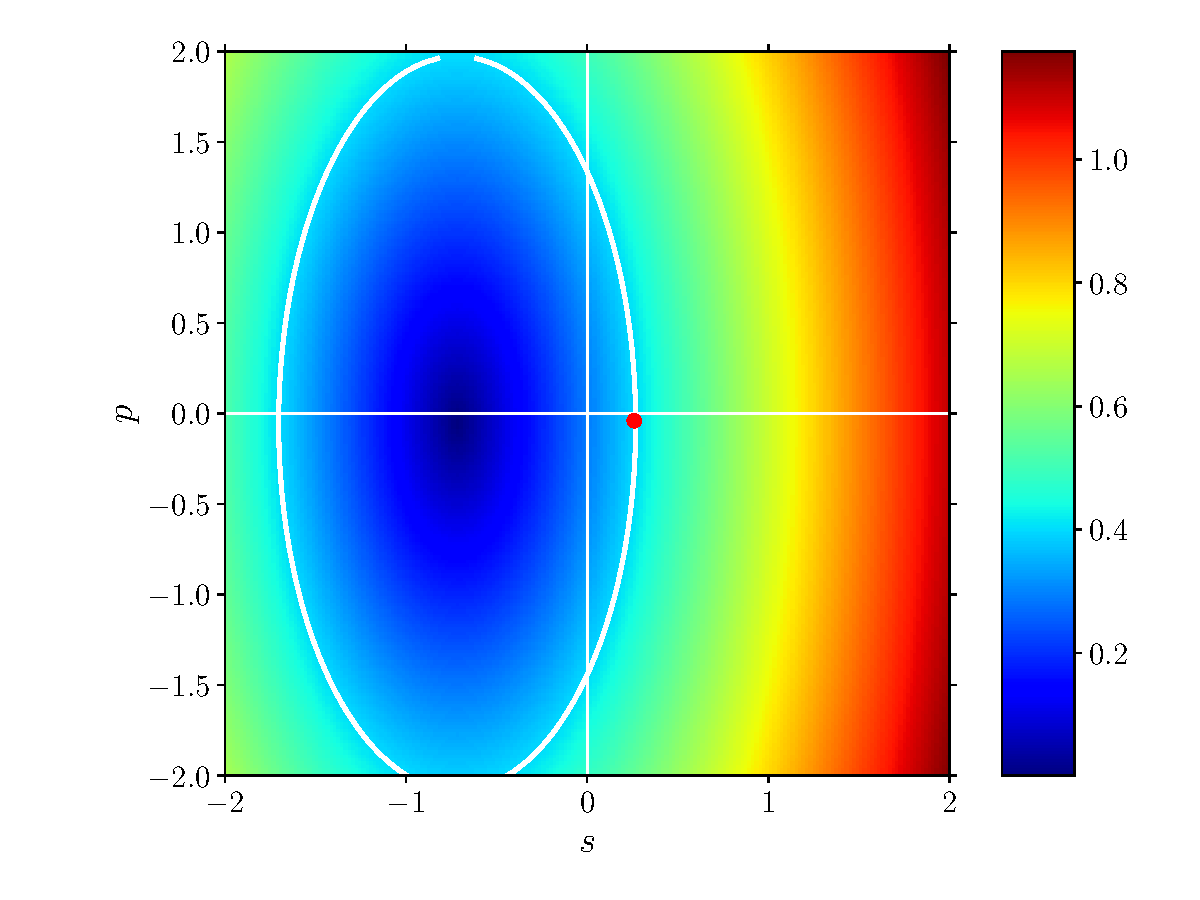
\includegraphics[width=\textwidth]{prestress_1_phase-diagram_eps.pdf}
        \subcaption{$\varepsilon$}
        \label{fig:}
    \end{minipage}
    \hfill
    \begin{minipage}[t]{.31\textwidth}
        \centering
        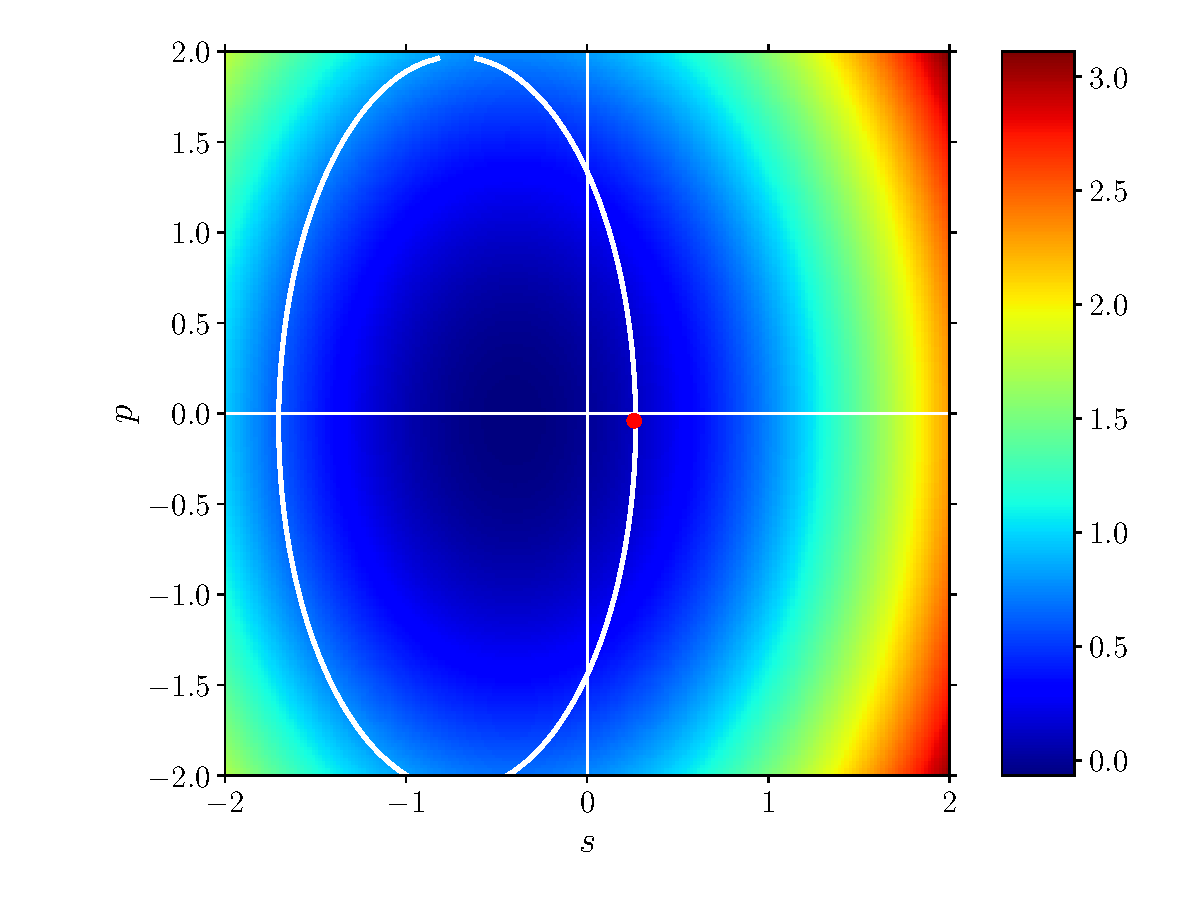
\includegraphics[width=\textwidth]{prestress_1_phase-diagram_energy.pdf}
        \subcaption{$\Delta E$}
        \label{fig:}
    \end{minipage}
    \hfill
    \begin{minipage}[t]{.31\textwidth}
        \centering
        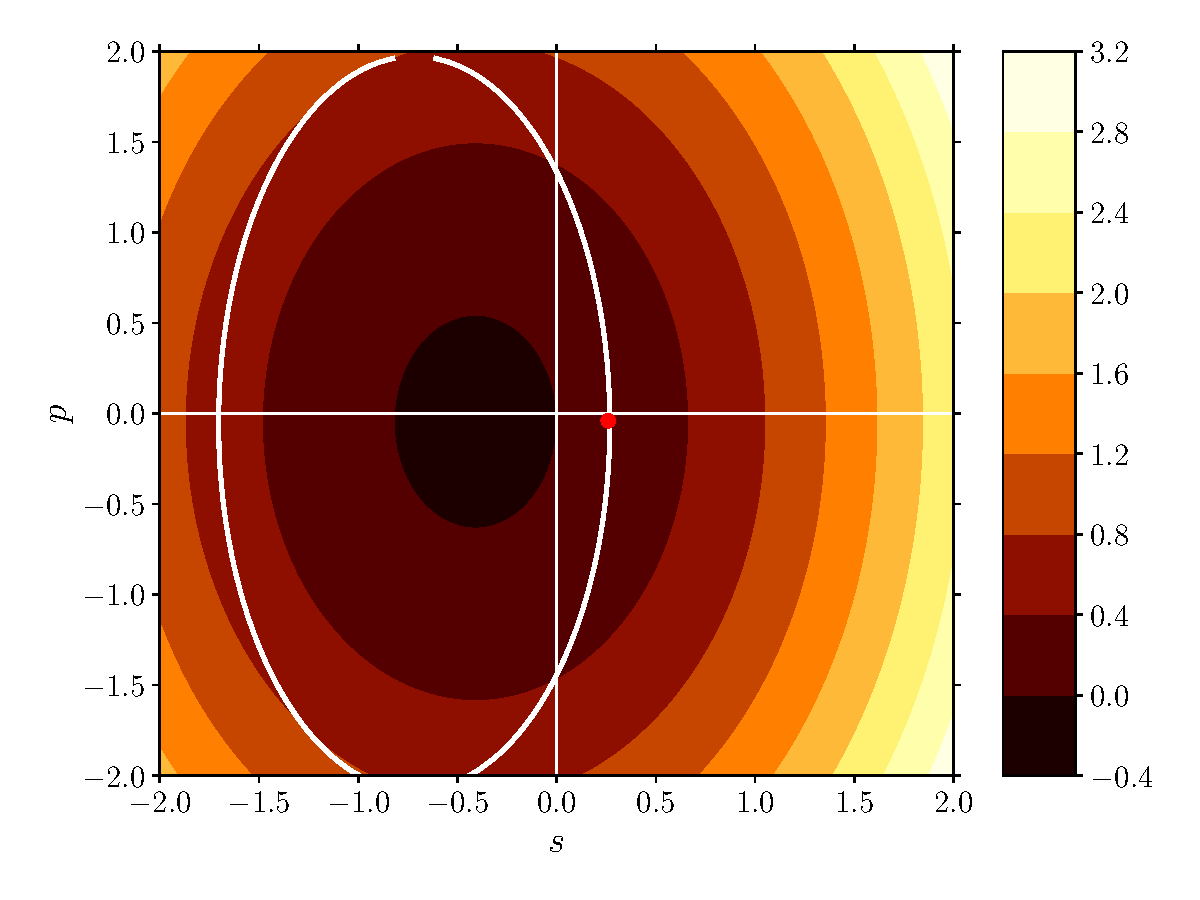
\includegraphics[width=\textwidth]{prestress_1_phase-diagram_energy-contour.pdf}
        \subcaption{$\Delta E$}
        \label{fig:}
    \end{minipage}
    \caption{Phase diagram for the configurations in \cref{fig:example:config}.}
    \label{fig:example:phase-diagram}
\end{figure}

\end{document}
